\documentclass[10pt]{exam}
\usepackage[phy]{template-for-exam}
\usepackage{graphicx,hyperref}

\title{Orbital Motion PhET Lab}
\author{Rohrbach}
\date{\today}

\begin{document}
\maketitle

\noindent
Go to \href{https://phet.colorado.edu/en/simulation/gravity-and-orbits}{\texttt{https://phet.colorado.edu/en/simulation/gravity-and-orbits}}.  Click on the “Play” button on the picture once on the appropriate page.  When open, click on the picture for the “model” option.

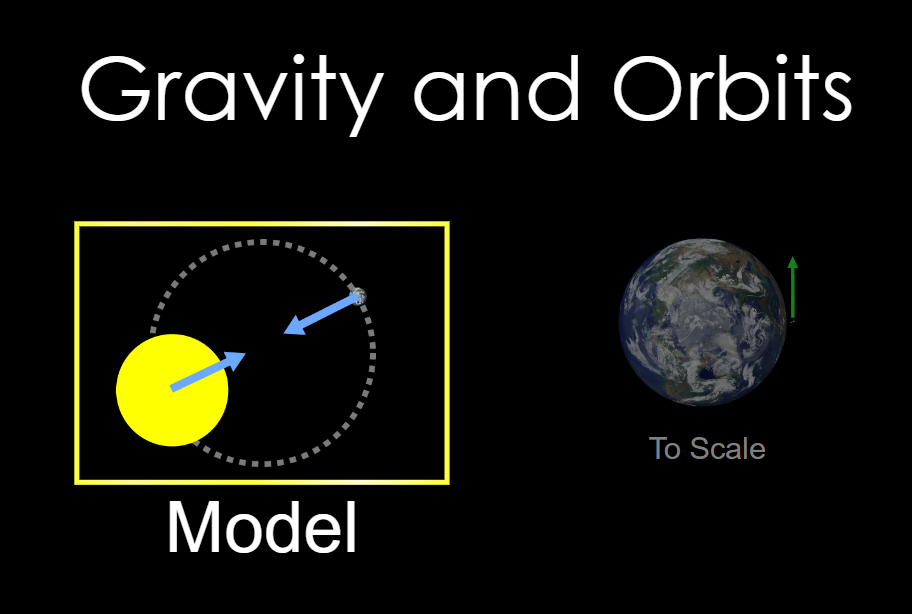
\includegraphics[width=4cm]{model.png} \hfill 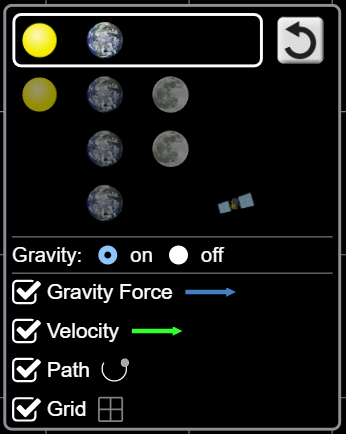
\includegraphics[width=3cm]{settings.png}

\begin{questions}

\question
  For the first demo you should have a simple Sun-Earth system (the first option).  Check ``on'' boxes for ``gravity force,'' ``velocity,'' ``path,'' and ``grid.''  Then click ``play.''

  

  \begin{parts}

    \part
      What force acting on the planet causes the centripetal force for this situation (think of forces we've talked about)?
      \vs

      % \begin{subparts}
      %   \subpart
      %     What force acting on the planet causes the centripetal force for this situation (think of forces we've talked about)?
      %     \vs
      %   \subpart
      %     If you watch the arrows closely, you will find that the force of gravity is a little bit stronger on the right side of the orbit than on the left side.  Why do you think this is?  
      %     \vs
      %   \subpart
      %     The speed of the earth is not perfectly constant.  Where is it going a little bit faster?  Why do you think this is?
      %     \vs
      % \end{subparts}
    
  \part
    If you look carefully, the Earth's path is not perfectly circular.  You can tell by using the grid to help.  This oblong circle shape is known as an \emph{ellipse}.  Explain why you think this orbit is not a perfect circle.
    \vs

  \part
    Adjust the velocity of the Earth by increasing and decreasing its velocity arrow.  Explain how this changes its motion around the Sun.
    \vs

  \part
    Increase the mass of the Sun to ``1.5'' and describe how and why the path of the Earth changes.
    \vs

  \part
    While the Earth is orbiting the Sun, switch gravity to “off” and explain how and why Earth's path changes.
    \vs

  \end{parts}

\pagebreak



\question
  Click ``reset'' and switch to the Sun-Earth-Moon system.  Make sure to turn back on the four checkboxes.

  \begin{parts}
    \part
    	Allow the moon and earth to orbit for a little bit.  Then, without stopping the animation, turn gravity ``off'' and explain the motion of both the Earth and the Moon.
      \vs

    \part
      Reset the Earth and Moon, and then drag the Moon away from the Earth.  Can you make it orbit the Sun instead?  Adjust velocity if needed.  What differences do you see about the force of gravity on the Moon?
      \vs
  \end{parts}


\question
  Click ``reset'' and select the Earth-Moon system.

  \begin{parts}
    \part
      Increase the mass of the Moon to ``2'' and click ``play.''  Explain what you notice about the motion of the Moon and the Earth.
      \vs

    \part
      The moon isn't the only thing moving.  The earth moves, too.  Why is this?  (\emph{Think about Newton's Laws.})
      \vs
    
  \end{parts}



\end{questions}


\end{document}